\documentclass[11pt]{article} 
\usepackage{amsmath}
\usepackage{amsfonts}
\usepackage{amssymb}
\usepackage{geometry}
\geometry{a4paper, margin=1in}
\usepackage{graphicx}
\usepackage[hidelinks]{hyperref}
\usepackage{amsthm}
\usepackage{tikz}
\usepackage{subcaption}
\usetikzlibrary{positioning}
\usepackage{pgfplots} 
\usepackage[ruled,vlined]{algorithm2e} 
\usepackage{dsfont}
\usepackage{graphicx}
\usepackage{mathdesign}
\usepackage{float}
\usepackage{todonotes} 
\usepackage{empheq}
\usepackage{array}
\usepackage[ruled,vlined]{algorithm2e} 
\usepackage[many]{tcolorbox}    	% for COLORED BOXES (tikz and xcolor included)



\newtcolorbox{boxA}{
    fontupper = \bf,
    boxrule = 1.5pt,
    colframe = black % frame color
}


\setlength{\parindent}{0pt}
\numberwithin{equation}{section}


\newcommand\mycommfont[1]{\footnotesize\ttfamily\textcolor{blue}{#1}}
\newcommand\defeq{\stackrel{\mathclap{\normalfont\mbox{def}}}{=}}
\SetCommentSty{mycommfont}

\DeclareMathOperator*{\argmax}{argmax}
\DeclareMathOperator*{\argmin}{argmin}



\newtheoremstyle{boldStyle}%                % Name
  {}%                                     % Space above
  {}%                                     % Space below
  {\itshape}%                                     % Body font
  {}%                                     % Indent amount
  {\bfseries}%                            % Theorem head font
  {}%                                    % Punctuation after theorem head
  {\newline}                              % Space after theorem head, new line
  {\thmname{#1}\thmnumber{ #2}\thmnote{ (#3)}}%                                     % Theorem head spec (can be left empty, meaning `normal')


\theoremstyle{boldStyle}
\newtheorem{example}{Example}[section]
\newtheorem{question}{Question}[section]
\newtheorem{answer}{Answer}[section]


\newtheorem*{claim*}{Claim}
\newtheorem*{lemma*}{Lemma}
\newtheorem*{corollary*}{Corollary}
\newtheorem*{remark*}{Remark}
\newtheorem*{example*}{Example}
\newtheorem*{examples*}{Examples}
\newtheorem*{definition*}{Definition}
\newtheorem*{question*}{Question}
\newtheorem*{answer*}{Answer}


\definecolor{blueColor}{rgb}{0, 0.611, 0.98} 
\newtheoremstyle{boldBlueStyle}%                % Name
  {}%                                          % Space above
  {}%                                          % Space below
  {\itshape}%                                  % Body font
  {}%                                          % Indent amount
  {\color{blueColor}\bfseries}%          % Theorem head font in red
  {}%                                          % Punctuation after theorem head
  {\newline}%                                  % Space after theorem head, new line
  {\thmname{#1}\thmnumber{ #2}\thmnote{ (#3)}} % Theorem head spec (can be left empty, meaning `normal')

\theoremstyle{boldBlueStyle}
\newtheorem{lemma}{Lemma}[section]
\newtheorem{corollary}{Corollary}[section]
\newtheorem{claim}{claim}[section]
\newtheorem{proposition}{Proposition}[section]



\definecolor{purpleColor}{rgb}{0.59, 0.223, 0.6} 
\newtheoremstyle{boldPurpleStyle}%                % Name
  {}%                                          % Space above
  {}%                                          % Space below
  {\itshape}%                                  % Body font
  {}%                                          % Indent amount
  {\color{purpleColor}\bfseries}%          % Theorem head font in red
  {}%                                          % Punctuation after theorem head
  {\newline}%                                  % Space after theorem head, new line
  {\thmname{#1}\thmnumber{ #2}\thmnote{ (#3)}} % Theorem head spec (can be left empty, meaning `normal')

\theoremstyle{boldPurpleStyle}
\newtheorem{theorem}{Theorem}[section]


\definecolor{redColor}{rgb}{1, 0.219, 0.219} 
\newtheoremstyle{boldRedStyle}%                % Name
  {}%                                          % Space above
  {}%                                          % Space below
  {\itshape}%                                  % Body font
  {}%                                          % Indent amount
  {\color{redColor}\bfseries}%          % Theorem head font in red
  {}%                                          % Punctuation after theorem head
  {\newline}%                                  % Space after theorem head, new line
  {\thmname{#1}\thmnumber{ #2}\thmnote{ (#3)}} % Theorem head spec (can be left empty, meaning `normal')

\theoremstyle{boldRedStyle}
\newtheorem{definition}{Definition}[section]




\title{
    \huge Probabilistic Methods in Artifical Intelligence\\
    \vspace{10pt}
}

\author{Hadar Tal}

\date{Hebrew University of Jerusalem, Israel\\
    \vspace{10pt}
    \today}



\begin{document}
\maketitle

\section{Probability Review}

\begin{definition}[Probability Space]
    A probability space is a triple $(\Omega, \mathcal{F}, P)$ where:
    \begin{enumerate}
        \item $\Omega$ is the sample space
        \item $\mathcal{F}$ is a $\sigma$-algebra of subsets of $\Omega$
        \item $P$ is a probability measure on $\mathcal{F}$ such that $P(\Omega) = 1$
    \end{enumerate}
\end{definition}

\begin{definition}[Joint Probability]
    The joint probability of two events $A$ and $B$ is:
    \begin{equation*}
        P(A, B) := P(A \cap B) 
    \end{equation*}
\end{definition}

\begin{definition}[Random Variable]
    A random variable $X$ is a function $X: \Omega \rightarrow \mathbb{R}$. 

    Val(X) = Image(X) = $\{ x \in \mathbb{R} : \exists \omega \in \Omega \text{ s.t. } X(\omega) = x \}$
\end{definition}

\begin{definition}[Probability Mass Function (PMF)]
    The probability mass function of a random variable $X$ is:
    \begin{equation*}
        P(X = x) := P(\{ \omega \in \Omega : X(\omega) = x \})
    \end{equation*}
\end{definition}

\begin{definition}[Joint Distribution]
    A joint distribution over a set of RVs $\mathcal{X} = \{ X_1, X_2, \ldots, X_n \}$ is a probability distribution 
    $P_{\mathcal{X}}: Val(X_1) \times Val(X_2) \times \ldots \times Val(X_n) \rightarrow [0, 1]$ defined by:
    \begin{equation*}
       \forall x_1, \ldots, x_n : x_i \in Val(X_i) \quad
        P_{\mathcal{X}}(x_1, x_2, \ldots, x_n) := P(X_1 = x_1, X_2 = x_2, \ldots, X_n = x_n)
    \end{equation*}
\end{definition}

\begin{proposition}[Law of Total Probability]
    For X, Y random variables, we can write:
    \begin{equation*}
        P(X) = \sum_{y \in Val(Y)} P(X, Y = y) 
    \end{equation*}
\end{proposition}

\begin{definition}[Conditional distribution]
    For X, Y RVs, and for any $y \in Val(Y)$ where $P(Y = y) > 0$ the conditional distribution of X given Y=y is:
    \begin{equation*}
        P(X| y) := \frac{P_{X,Y}(X = x, Y = y)}{P_Y(Y = y)}
    \end{equation*}
\end{definition}

\begin{proposition}[Chain Rule]
    For any set of random variables $X_1, X_2, \ldots, X_n$:
    \begin{equation*}
        P(X_1, X_2, \ldots, X_n) = P(X_1)P(X_2 | X_1)P(X_3 | X_1, X_2) \ldots P(X_n | X_1, X_2, \ldots, X_{n-1})
    \end{equation*}
\end{proposition}

\begin{proposition}[Bayes' Rule]
    For any two random variables $H, E$:
    \begin{equation*}
       P(H = h | E = e) = \frac{P(E = e | H = h)P(H = h)}{P(E = e)}
    \end{equation*}
    where we often call:
    \begin{itemize}
        \item $P(H = h)$ the \textbf{prior} probability
        \item $P(H = h | E = e)$ the \textbf{posterior} probability in light of evidence $E = e$
        \item $P(E = e | H = h)$ the \textbf{likelihood} of the evidence $E = e$ given the hypothesis $H = h$
    \end{itemize}
\end{proposition}

\begin{definition}[Marginal Independence]
    Let $P$ be a probability distribution over a set of random variables $\mathcal{X}$ and let $X, Y \in \mathcal{X}$.
    We say that $X$ is independent of $Y$, denoted $P \models X \perp Y$, if
    \begin{equation*}
        P(X | Y) = P(X)
    \end{equation*}
\end{definition}

\begin{definition}[Conditional Independence]
    Let $P$ be a probability distribution over a set of random variables $\mathcal{X}$ and let $X, Y, Z \in \mathcal{X}$.
    We say that $X$ is independent of $Y$ given $Z$, denoted $P \models X \perp Y | Z$, if
    \begin{equation*}
        P(X | Y, Z) = P(X | Z)
    \end{equation*}
\end{definition}

\begin{lemma}[Equivalent Definitions of Conditional Independence]
    Let $P$ be a probability distribution over a set of random variables $\mathcal{X}$ and let $X, Y, Z \in \mathcal{X}$.
    The following are equivalent:
    \begin{enumerate}
        \item $P \models X \perp Y | Z$
        \item $P(X, Y | Z) = P(X | Z) P(Y | Z)$
        \item $P(X, Y, Z) = P(X | Z) P(Y , Z)$
        \item $\exists f, g : P(X, Y, Z) = f(X, Z)g(Y, Z)$
    \end{enumerate}
\end{lemma}

\begin{theorem}[Properties of Conditional Independence]
    Let $P$ be a probability distribution over a set of random variables $\mathcal{X}$ and let $X, Y, Z, W \in \mathcal{X}$.
    The following hold:
    \begin{enumerate}
        \item \textbf{Symmetry} - $(X \perp Y | Z) \implies (Y \perp X | Z)$
        \item \textbf{Decomposition} - $(X \perp Y, W | Z) \implies (X \perp Y | Z) \land (X \perp W | Z)$
        \item \textbf{Weak Union} - $(X \perp Y, W | Z) \implies (X \perp Y | W, Z)$
        \item \textbf{Contraction} - $(X \perp Y | Z) \land (X \perp W | Y, Z) \implies (X \perp Y, W | Z)$
        \item \textbf{Intersection} - For \textit{strictly positive} distributions, 
            \[(X \perp Y | W, Z) \land (X \perp W | Y, Z) \implies (X \perp Y, W | Z)\]
    \end{enumerate}
\end{theorem}







% * * * * * * * * * * * * * * * * * * * * * * * * 
% * * * * * * * * * * * * * * * * * * * * * * * * 
% * * * * * * * * * * * * * * * * * * * * * * * * 
% * * * * * * * * * * * * * * * * * * * * * * * * 
% * * * * * * * * * * * * * * * * * * * * * * * * 
% * * * * * * * * * * * * * * * * * * * * * * * * 
% * * * * * * * * * * * * * * * * * * * * * * * * 
% * * * * * * * * * * * * * * * * * * * * * * * * 
% * * * * * * * * * * * * * * * * * * * * * * * * 
% * * * * * * * * * * * * * * * * * * * * * * * * 
% * * * * * * * * * * * * * * * * * * * * * * * * 
% * * * * * * * * * * * * * * * * * * * * * * * * 
% * * * * * * * * * * * * * * * * * * * * * * * * 
% * * * * * * * * * * * * * * * * * * * * * * * * 
% * * * * * * * * * * * * * * * * * * * * * * * * 
% * * * * * * * * * * * * * * * * * * * * * * * * 
% * * * * * * * * * * * * * * * * * * * * * * * * 
% * * * * * * * * * * * * * * * * * * * * * * * * 
% * * * * * * * * * * * * * * * * * * * * * * * * 
\newpage
\section{Bayesian Networks}

\subsection{Bayesian Networks Basics}

\begin{definition}[Probabilistic Graphical Model (PGM)]
    A probabilistic graphical model is a pair $(\mathcal{G}, P)$ where:
    \begin{enumerate}
        \item $\mathcal{G}$ is a graph
        \item $P$ is a probability distribution
    \end{enumerate}
\end{definition}

\begin{definition}[Bayesian Network]
    A Bayesian Network $\mathcal{B}$ is:
    \begin{enumerate}
        \item \textbf{Bayesian Network Structure} - A directed acyclic graph (DAG) $\mathcal{G} = (\mathcal{X}, E)$  ($|\mathcal{X}| = n$)
        \item \textbf{Set of CPDs} - $\{ P_i(X_i | \text{Pa}(X_i) ) \}_{i=1}^{n}$ 
    \end{enumerate}
    the network defines a probability distribution: 
    \begin{equation*}
        P_{\mathcal{B}}(X_1, X_2, \ldots, X_n) = \prod_{i=1}^{n} P_i(X_i | \text{Pa}(X_i))
    \end{equation*}
    A Bayesian Network is the tuple $\mathcal{B} = (\mathcal{G}, P_{\mathcal{B}})$.
\end{definition}

\begin{theorem}[Bayesian Network defines a probability distribution]
    For any Bayesian Network $B$, $P_B(X_1, X_2, \ldots, X_n)$ is a joint probability distribution over the variables $X_1, X_2, \ldots, X_n$.
\end{theorem}

\begin{definition}[Descendants of a node]
    Let $G = (V, E)$ be a directed graph and let $X_i \in V$. The descendants of $X_i$ are: 
    \begin{equation*}
        D(X_i) = \{ X_j \in \mathcal{X} : \exists \text{ directed path } X_i \rightarrow \cdots \rightarrow  X_j \}
    \end{equation*}
\end{definition}

\begin{definition}[Naive Bayes Model]
    A Naive Bayes Model is a Bayesian Network where all the features are non adjacent children of the class node.
\end{definition}

\begin{definition}[Naive Bayes Classifier]
    A Naive Bayes Classifier is a classifier that uses the Naive Bayes Model to classify instances.
    \[
        \hat{c} = \argmax_{c \in C} { P(c | x_1, x_2, \ldots, x_n) } = \argmax_{c \in C} { P(c, x_1, x_2, \ldots, x_n) } = \argmax_{c \in C} { P(c) \prod_{i=1}^{n} P(x_i | c) }
    \]
\end{definition}

\subsection{Independencies and Factorization in Bayesian Networks}

\begin{definition}[$I_{LM}(\mathcal{G})$]
    The \textbf{Local Markov Independencies Set} of a Bayesian Network $B$ is the set of all independencies that hold in the network:
    \begin{equation*}
        I_{LM}(\mathcal{G}) = \{ (X_i \perp ND(X_i) | \text{Pa}(X_i))\}_{i=1}^{|\mathcal{X}|}
    \end{equation*}
\end{definition}

\begin{definition}[I(P)]
    The set of independencies that hold in a distribution $P$ over $\mathcal{X}$ is:
    \begin{equation*}
        I(P) = \{(X \perp Y | Z) :  (X,Y,Z) \subseteq \mathcal{X} , \quad  P \models (X \perp Y | Z)  \}
    \end{equation*}
\end{definition}

\begin{definition}[I-map]
    A DAG $\mathcal{G}$ is an I-map of a distribution $P$ if all independencies assumptions of $\mathcal{G}$ hold in $P$:
    \begin{equation*}
        I_{LM}(\mathcal{G}) \subseteq I(P)
    \end{equation*}
\end{definition}

\begin{theorem}[Factorization]
    If $G$ is an I-map of $P$, then we can write:
    \begin{equation*}
        P(X_1, X_2, \ldots, X_n) = \prod_{i=1}^{n} P(X_i | \text{Pa}(X_i))
    \end{equation*}
\end{theorem}

\begin{definition}[Factorization]
    We say that $P$ factorizes over $\mathcal{G}$ if there exist CPDs $\{ P_i \}_{i=1}^{n}$ such that:
    \begin{equation*}
        P(X_1, X_2, \ldots, X_n) = \prod_{i=1}^{n} P_i(X_i | \text{Pa}(X_i))
    \end{equation*}
\end{definition}

\begin{corollary}[Independencies implies Factorization]
    If $\mathcal{G}$ is an I-map of $P$ ($P \models I_{LM}(\mathcal{G})$), then $P$ factorizes over $\mathcal{G}$.
\end{corollary}

\begin{corollary}[Independencies implies Factorization (2)]
    If $\mathcal{G}$ is an I-map of $P$ ($P \models I_{LM}(\mathcal{G})$), then $(\mathcal{G}, P)$ is a Bayesian Network.
\end{corollary}

\begin{theorem}[Independencies in $P_B$]
    For $P_\mathcal{B}$ it holds for all $i$ that
    \begin{enumerate}
        \item $X_i \perp ND(X_i) | \text{Pa}(X_i)$  \quad  ($I_{LM}(\mathcal{G})$)
        \item $P_\mathcal{B}(X_i | ND(X_i)) = P_i(X_i | \text{Pa}(X_i))$
    \end{enumerate}
\end{theorem}

\begin{corollary}[Factorization implies Independencies]
    If $P$ factorizes over $\mathcal{G}$, then $\mathcal{G}$ is an I-map of $P$ ($P \models I_{LM}(\mathcal{G})$).
\end{corollary}

\begin{theorem}[Fundmental Theorem of Bayesian Networks]
    Let $\mathcal{G}$ be a BN structure over $\mathcal{X} = {X_1, X_2, \ldots, X_n}$ and let $P$ be a joint distribution over $\mathcal{X}$. 
    
    Then $\mathcal{G}$ is an I-map of $P$ $\Leftrightarrow$ $P$ factorizes over $\mathcal{G}$.
\end{theorem}

\begin{definition}[Minimal I-map]
    A DAG $\mathcal{G}$ is a minimal I-map of a distribution $P$ if 
    \begin{enumerate}
        \item $\mathcal{G}$ is an I-map of $P$
        \item If $\mathcal{G}' \subset \mathcal{G}$ then $\mathcal{G}'$ is not an I-map of $P$
    \end{enumerate}
\end{definition}


\subsection{Reasoning Patterns in Bayesian Networks}


\begin{definition}[Reasoning Patterns in Bayesian Networks]
    There are 4 main reasoning patterns in Bayesian Networks:
    \begin{itemize}
        \item \textbf{Downstream (causal) reasoning} - $X \rightarrow Z \rightarrow Y$
        \item \textbf{Upstream (evidential) reasoning} - $X \leftarrow Z \leftarrow Y$
        \item \textbf{Common Causal reasoning} - $X \leftarrow Z \rightarrow Y$
        \item \textbf{Common Effect reasoning} - $X \rightarrow Z \leftarrow Y$
    \end{itemize}
\end{definition}

\begin{figure}[H]
    \centering 
    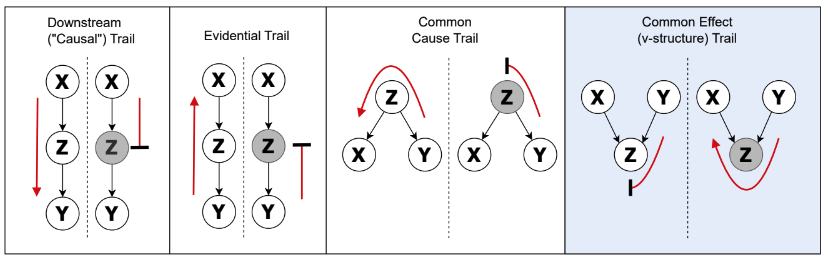
\includegraphics[width=0.9\textwidth]{figs/reasoning_in_BN.png}
    \label{fig:reasoning_in_BN}
    \caption{Reasoning Patterns in Bayesian Networks}
\end{figure}


\subsection{D-separation}

\begin{question}
    If $P$ factorizes over $\mathcal{G}$, then $\mathcal{G}$ is an I-map of $P$ ($P \models I_{LM}(\mathcal{G})$).

    Can p satisfy more independencies than those implied by $\mathcal{G}$? Yes. 

    Given $\textbf{X}, \textbf{Y}, \textbf{Z}\in \mathcal{X}$, we would like to characterize when does $P \models I_{LM}(\mathcal{G}) \implies P \models X \perp Y | Z$.

    Or characterize the complement - Can we find $P$ that factorizes over $\mathcal{G}$ but $P \not\models X \perp Y | Z$?

\end{question}

\begin{definition}[Active Trail]
    A trail $X = X_1 - X_2 - \cdots - X_n$ between X and Y in a BN is active given a set of observed RVs $Z$,
    if whenever there is a v-structure along the trail $X_{i-1} \rightarrow X_{i} \leftarrow X_{i+1}$, then $X_{i}$ or one of its descendants is in $Z$, 
    and all other nodes along the trail are not in $Z$.
\end{definition}

\begin{definition}[d-separation]
    The sets $\textbf{X}$ and $\textbf{Y}$ are d-separated given $\textbf{Z}$ in $\mathcal{G}$, denoted $\text{d-sep}_{\mathcal{G}}(\textbf{X};\textbf{Y} | \textbf{Z})$,
    if there is no active trail between any node in $\textbf{X}$ and any node in $\textbf{Y}$ given $\textbf{Z}$.
\end{definition}

\begin{definition}[Global Markov Independencies]
    The set of global Markov Independencies of a BN structure $\mathcal{G}$ is the set of all independencies that correspond to d-separation:
    \begin{equation*}
        I(\mathcal{G}) := I_{GM}(\mathcal{G}) := \{ (X \perp Y | Z) : \text{d-sep}_{\mathcal{G}}(X;Y | Z) \}
    \end{equation*}
    d-separation characterizes precisely the full set of independencies that a BN structure encodes.
\end{definition}

\begin{theorem}[Soundness]
    If a distribution $P$ factorizes over a BN structure $\mathcal{G}$, then $I(\mathcal{G}) \subseteq I(P)$.
\end{theorem}
Note - the other direction is not true. If a distribution $P$ factorizes over $\mathcal{G}$, then it is not necessarily true that $I(P) \subseteq I(\mathcal{G})$.

\begin{theorem}[completness]
    If $(X \perp Y | Z) \notin I(\mathcal{G})$, then there exists a distribution $P$ that factorizes over $\mathcal{G}$ in which 
    
    $P \not\models (X \perp Y | Z)$.
\end{theorem}




% * * * * * * * * * * * * * * * * * * * * * * * * 
% * * * * * * * * * * * * * * * * * * * * * * * * 
% * * * * * * * * * * * * * * * * * * * * * * * * 
% * * * * * * * * * * * * * * * * * * * * * * * * 
% * * * * * * * * * * * * * * * * * * * * * * * * 
% * * * * * * * * * * * * * * * * * * * * * * * * 
% * * * * * * * * * * * * * * * * * * * * * * * * 
% * * * * * * * * * * * * * * * * * * * * * * * * 
% * * * * * * * * * * * * * * * * * * * * * * * * 
% * * * * * * * * * * * * * * * * * * * * * * * * 
% * * * * * * * * * * * * * * * * * * * * * * * * 
% * * * * * * * * * * * * * * * * * * * * * * * * 
% * * * * * * * * * * * * * * * * * * * * * * * * 
% * * * * * * * * * * * * * * * * * * * * * * * * 
% * * * * * * * * * * * * * * * * * * * * * * * * 
% * * * * * * * * * * * * * * * * * * * * * * * * 
% * * * * * * * * * * * * * * * * * * * * * * * * 
% * * * * * * * * * * * * * * * * * * * * * * * * 
% * * * * * * * * * * * * * * * * * * * * * * * * 
\newpage
\section{Bayesian Networks}


\end{document}